\documentclass[journal,12pt,twocolumn]{IEEEtran}

\usepackage{setspace}
\usepackage{gensymb}
\singlespacing
\usepackage[cmex10]{amsmath}

\usepackage{amsthm}

\usepackage{mathrsfs}
\usepackage{txfonts}
\usepackage{stfloats}
\usepackage{bm}
\usepackage{cite}
\usepackage{cases}
\usepackage{subfig}

\usepackage{longtable}
\usepackage{multirow}
\usepackage{enumitem}
\usepackage{mathtools}
\usepackage{steinmetz}
\usepackage{tikz}
\usepackage{circuitikz}
\usepackage{verbatim}
\usepackage{tfrupee}
\usepackage[breaklinks=true]{hyperref}
\usepackage{graphicx}
\usepackage{tkz-euclide}

\usetikzlibrary{calc,math}
\usepackage{listings}
    \usepackage{color}                                            %%
    \usepackage{array}                                            %%
    \usepackage{longtable}                                        %%
    \usepackage{calc}                                             %%
    \usepackage{multirow}                                         %%
    \usepackage{hhline}                                           %%
    \usepackage{ifthen}                                           %%
    \usepackage{lscape}     
\usepackage{multicol}
\usepackage{chngcntr}

\DeclareMathOperator*{\Res}{Res}

\renewcommand\thesection{\arabic{section}}
\renewcommand\thesubsection{\thesection.\arabic{subsection}}
\renewcommand\thesubsubsection{\thesubsection.\arabic{subsubsection}}

\renewcommand\thesectiondis{\arabic{section}}
\renewcommand\thesubsectiondis{\thesectiondis.\arabic{subsection}}
\renewcommand\thesubsubsectiondis{\thesubsectiondis.\arabic{sub subsection}}


\hyphenation{optical networks semiconduc-tor}
\def\inputGnumericTable{}                                 %%

\lstset{
%language=C,
frame=single, 
breaklines=true,
columns=fullflexible
}
\date{March 2021}

\begin{document}

\newcommand{\BEQA}{\begin{eqnarray}}
\newcommand{\EEQA}{\end{eqnarray}}
\newcommand{\define}{\stackrel{\triangle}{=}}
\bibliographystyle{IEEEtran}
\raggedbottom
\setlength{\parindent}{0pt}
\providecommand{\mbf}{\mathbf}
\providecommand{\pr}[1]{\ensuremath{\Pr\left(#1\right)}}
\providecommand{\qfunc}[1]{\ensuremath{Q\left(#1\right)}}
\providecommand{\fn}[1]{\ensuremath{f\left({#1}\right)}}
\providecommand{\e}[1]{\ensuremath{E\left(#1\right)}}
\providecommand{\sbrak}[1]{\ensuremath{{}\left[#1\right]}}
\providecommand{\lsbrak}[1]{\ensuremath{{}\left[#1\right.}}
\providecommand{\rsbrak}[1]{\ensuremath{{}\left.#1\right]}}
\providecommand{\brak}[1]{\ensuremath{\left(#1\right)}}
\providecommand{\lbrak}[1]{\ensuremath{\left(#1\right.}}
\providecommand{\rbrak}[1]{\ensuremath{\left.#1\right)}}
\providecommand{\cbrak}[1]{\ensuremath{\left\{#1\right\}}}
\providecommand{\lcbrak}[1]{\ensuremath{\left\{#1\right.}}
\providecommand{\rcbrak}[1]{\ensuremath{\left.#1\right\}}}
\theoremstyle{remark}
\newtheorem{rem}{Remark}
\newcommand{\sgn}{\mathop{\mathrm{sgn}}}
\newcommand{\comb}[2]{{}^{#1}\mathrm{C}_{#2}}
\providecommand{\abs}[1]{\vert#1\vert}
\providecommand{\res}[1]{\Res\displaylimits_{#1}} 
\providecommand{\norm}[1]{\lVert#1\rVert}
%\providecommand{\norm}[1]{\lVert#1\rVert}
\providecommand{\mtx}[1]{\mathbf{#1}}
\providecommand{\mean}[1]{E\sbrak{ #1 }}
\providecommand{\fourier}{\overset{\mathcal{F}}{ \rightleftharpoons}}
%\providecommand{\hilbert}{\overset{\mathcal{H}}{ \rightleftharpoons}}
\providecommand{\system}{\overset{\mathcal{H}}{ \longleftrightarrow}}
	%\newcommand{\solution}[2]{\textbf{Solution:}{#1}}
\newcommand{\solution}{\noindent \textbf{Solution: }}
\newcommand{\cosec}{\,\text{cosec}\,}
\providecommand{\dec}[2]{\ensuremath{\overset{#1}{\underset{#2}{\gtrless}}}}
\newcommand{\myvec}[1]{\ensuremath{\begin{pmatrix}#1\end{pmatrix}}}
\newcommand{\mydet}[1]{\ensuremath{\begin{vmatrix}#1\end{vmatrix}}}
\numberwithin{equation}{subsection}
\makeatletter
\vspace{3cm}
\title{EE3900 Gate Assignment - 1}
\author{Adhvik Mani Sai Murarisetty - AI20BTECH11015}
\maketitle
\newpage
\bigskip
\renewcommand{\thetable}{\theenumi}

%
Download latex-tikz codes from 
%
\begin{lstlisting}
https://github.com/adhvik24/EE3900/blob/main/Assignment_1/Final_Assignment_1.tex
\end{lstlisting}
\section{Gate EC 2018 Qn 54}
A band limited low-pass signal x(t) of bandwidth 5 kHz is sampled at a sampling rate $f_s$.
The signal x(t) is reconstructed using the reconstruction filter H(f) whose magnitude response is shown below:

\begin{figure}[htp]
    \centering
    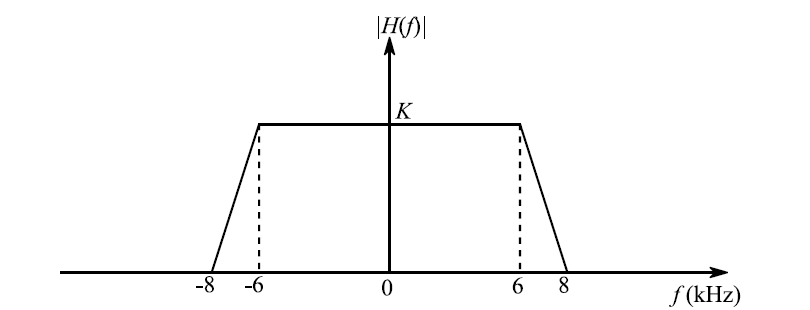
\includegraphics[width=\columnwidth]{gate_1_1.PNG}
\end{figure}

The minimum sampling rate $f_s$ (in kHz) for perfect reconstruction of x(t) is
\section{SOLUTION}
As x(t) is a band limited low-pass signal of bandwidth 5kHz.

Let our signal x(t) be look like,
\begin{figure}[htp]
    \centering
    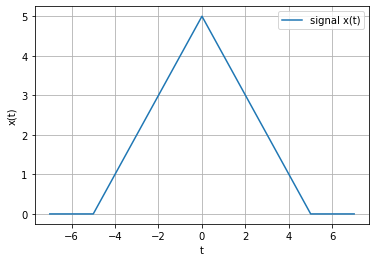
\includegraphics[width=\columnwidth]{gate_1_2.png}
\end{figure}

After sampling x(t) at a sampling rate of $f_s$, Then it signal looks like a repetitive triangular wave that repeats after $f_s$kHz.
Then the sampled signal s(t) looks like,
\begin{figure}[htp]
    \centering
    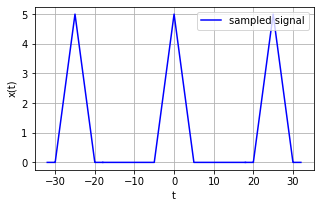
\includegraphics[width=\columnwidth]{gate_sample.png}
    \caption{Sampled signal}
\end{figure}

\textbf{Note: Here for plotting $f_s$ has been taken as 25kHz.}

On applying the given reconstruction filter on the sampled signal looks like,
(When $f_s$ = 25kHz)
\begin{figure}[htp]
    \centering
    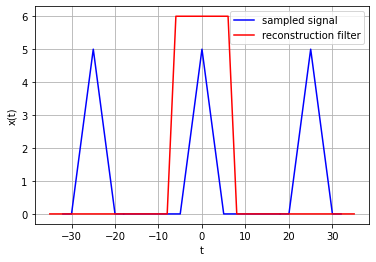
\includegraphics[width=\columnwidth]{gate_fiter.png}
    \caption{Applying filter on sampled signal
    \\\textbf{Note: Here for plotting $f_s$ has been taken as 25kHz.}}
\end{figure}

We are observing a perfect reconstruction of x(t) is possible in the case of $f_s$=25kHz.

But if we observe when $f_s$=11kHz, It is not possible to perfect reconstruction of x(t). As it looks like ,
\begin{figure}[htp]
    \centering
    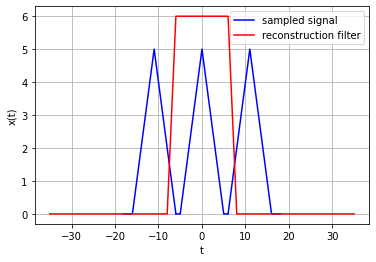
\includegraphics[width=\columnwidth]{gate_filter_1.png}
    \caption{Applying filter on sampled signal
    \\\textbf{Note: Here for plotting $f_s$ has been taken as 11kHz.}}
\end{figure}
\newpage
Therefore, The condition for perfect reconstruction of x(t) from s(t) using filter H is,
$$f_m\le f_H\le f_s-f_m$$

Where $f_m$ is the maximum component frequency of x(t), $f_H$ is that of filter and $f_s$ is the sampling frequency.

We know the $f_m$ is 5kHz,$f_H$ is 8kHz and the next sampled part signal starts at $f_s$-5 kHz.

For perfect reconstruction of x(t) which has been sampled at a rate $f_s$, $$f_s-5 \ge 8$$
So, The possible values of $f_s$ for which reconstruction of x(t) possible is 
$$f_s \ge 13$$
$\therefore$ The minimum sampling rate $f_s$ for perfect reconstruction of x(t) is 13kHz.

\end{document}
